\section{Results}

\subsection{Datasets}\label{sec:results:data}

%\mdeff{All stuff about data here.
%Ideally same data for all experiments.}
%\todo{Merge and shorten.}
%\todo{$P$ training projections.}

%\paragraph{Proteins.}
We consider two proteins: the $\beta$-galactosidase, a protein with a dihedral (D2) symmetry, and the lambda excision HJ intermediate (HJI), an asymmetric protein.
Their deposited PDB atomic models are \texttt{5a1a}~\cite{bartesaghi2015betagal} and \texttt{5j0n}~\cite{laxmikanthan2016structure}, respectively.
For each atomic model, we generate the ground truth by fitting a 5\AA\ density map in Chimera~\cite{pettersen2004ucsf}.
We thus obtain a volume of $110 \times 155 \times 199$ voxels for the $\beta$-galactosidase, and a volume of size $69 \times 57 \times 75$ voxels for the HJI.

\paragraph{Projections.}
From these ground truths, we generate $5,000$ synthetic projections of size $275\times 275$ and $116\times 116$, respectively, using the ASTRA projector~\cite{van2015astra}.
Our projection generator has a support for two different projection orientation sampling methods: (1) sampling uniformly the Euler angles and (2) sampling uniformly on $\textbf{SO}(3)$ space. Due to protein symmetries, in the experiments that follow, the asymmetric protein \texttt{5j0n} has a half-$\mathbb{S}^2$-sphere coverage, and the symmetric protein \texttt{5a1a} has a quarter-$\mathbb{S}^2$-sphere coverage.
\figref{different-projections} shows example projections.

\begin{figure}[ht!]
    \centering
    \begin{subfigure}[b]{0.3\textwidth}
        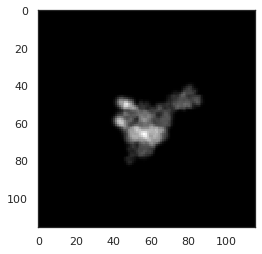
\includegraphics[height=4cm]{images/5j0n_noise0.png}
        \caption{}
    \end{subfigure}
    \hfill
    \begin{subfigure}[b]{0.3\textwidth}
    \centering
        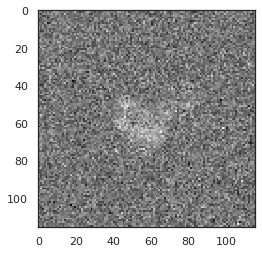
\includegraphics[height=4cm]{images/5j0n_noise16.png}
        \caption{}
    \end{subfigure}
    \hfill
    \begin{subfigure}[b]{0.3\textwidth}
    \centering
        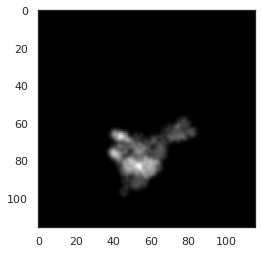
\includegraphics[height=4cm]{images/5j0n_translated.png}
        \caption{}
    \end{subfigure}
    \caption{An example projection being perturbed.
    \textbf{(a)} \mdeff{Clean (better word?)} projection.
    \textbf{(b)} With additive white noise of variance 16.
    \textbf{(c)} Translated with triangle distribution from -20 to 20 pixels, and peak at 0.}
    \label{fig:different-projections}
\end{figure}

\paragraph{Perturbations.}
\mdeff{Better word?}
We consider the following perturbations to control the difficulty of orientation recovery: (i) additive white noise, (ii) translations, (iii) point-spread functions (PSF).
We consider that a cryo-EM measurement (i.e. projection) $\mathbf{p}_i \in \mathbb{R}^{M}$ is acquired through
\begin{equation}
\label{eq:linear-forward-model}
\mathbf{p}_i={\mathbf {C}_{\boldsymbol\varphi}}\mathbf S_{\mathbf{t}}\mathbf P_{\theta_i}\mathbf x+\mathbf n,
\end{equation}
where $\mathbf x \in \mathbb{R}^{V}$ is the unknown 3D density map\cite{dimaio_creating_2007} (Coulomb potential). The operator $\mathbf P_{\theta_i}: \mathbb R^V \to \mathbb R^M$ is the projection along the 3D pose $\theta_i$ (i.e., the x-ray transform). The operator $\mathbf S_\mathbf{t}: \mathbb R^M \to \mathbb R^M$ is a shift of the projection by $\mathbf{t}=(t_1, t_2)$. The convolution operator $\mathbf {C}_{\boldsymbol\varphi}: \mathbb R^M \to \mathbb R^M$ models the microscope contrast transfer function (CTF) with parameters $\boldsymbol\varphi=(d_1, d_2, \alpha_{\rm ast})$, that are, respectively, the defocus-major, the defocus-minor and the angle of astigmatism. Finally, $\mathbf n \in \mathbb{R}^{M}$ represents an additive noise. Our goal is then to recover the angles $\theta_i$ from every projection $\mathbf y_i$.

\begin{table}[ht!]
    \centering
    \begin{tabular}{lrrr}
        \toprule
        Dataset & Number of projections $P$ (\%) & Maximum number of pairs $P^2$ & Used number of pairs \\
        \midrule
        Train set & 2512 (50\%) & 6,312,656 & 63,126 (1\%) \\
        Validation set & 1650 (33\%) & 2,722,500 & 27,225 (1\%) \\
        Test set & 837 (17\%) & 701,406 & randomly sampled per batch \\
        \bottomrule
    \end{tabular}
    \caption{Training, validation, and test datasets.}\label{tab:dataset}
\end{table}

\paragraph{Distance learning.}
We use supervised learning, thus input-output pairs.
The input are two images and the output is their quaternion distance calculated from the ground truth orientations.
For neural network training, dataset is split into a distinct training, validation, and testing set, see \tabref{dataset}, to ensure that the results can generalize to unseen projections.


\paragraph{Orientation recovery.}
The orientation recovery is solving \eqnref{orientation-recovery} and it was done in a stochastic setting, where the loss function varies over the batches.
Hence, the dataset used in this part is test set from \tabref{dataset}.
Orientation recovery is performed on projections unseen during distance learning.

\subsection{Evaluation}\label{sec:results:evaluation}

%\mdeff{Story: need to know how good we did (without reconstructing the protein).
%As orientations are up to a global rotation/mirror on $\SO(3) / \mathbb{S}^3$, best align recovered and true orientations before computing the mean recovery error.}

%\todo{Introduce the mean recovery error as a good and intuitive performance metric.}
%\todo{Figure that shows a typical convergence and mean orientation recovery error before and after alignment. We'll subsequently only report $E$ (the error after alignment).}

Before discussing the results, we remark that one cannot really quantify the performance of~\eqnref{orientation-recovery} through its loss nor visual judgement of the protein reconstruction.
Unfortunately, it is also not appropriate to directly compute the error between the recovered orientations $\big\{\widehat{q}_p\big\}_{p=1}^P$ and the true ones $\big\{q_p\big\}_{p=1}^P$.
The reason is that the recovery of orientation through~\eqnref{orientation-recovery} is up to a global rotation, \textit{i.e.}, any global rotation of the set of recovered orientations is as valid as any other.
This is not a problem for the ultimate application of our scheme, but it complicates the quantitative evaluation of its performance in synthetic experiments.
We circumvent this problem by aligning the true and recovered orientation sets up to a global rotation and mirror on $SO(3)$ space \textit{i.e.} objective is to minimize the distance difference between these two sets.


The goal of the alignment is to compute the \textit{mean orientation recovery error}
\begin{equation}
    E = \min_{\T \in \Or(4)} \frac{1}{P_{test}} \sum_{i} \big| d_q\left( q_i, \T \hat{q_i} \right) \big|,
    \label{eqn:orientation-recovery-error}
\end{equation}
where $\Or(4) = \{\T | \det(\T) = \pm 1\}$ is the group of $4 \times 4$ orthogonal matrices that represent 4D rotations and reflections/mirrors \textit{i.e.} it consists of proper and improper rotations, and $P_{test}$ is the number of projections in test set.
In practice, the sum is again sampled and \eqnref{orientation-recovery-error} is separately minimized using gradient descent method with FTRL optimizer \cite{mcmahan_ad_2013,noauthor_tfkerasoptimizersftrl_nodate} for $\det(\T) = 1$ (proper rotations) and $\det(\T) = -1$ (improper rotations) because $\Or(4)$ is disconnected.

We implement $\T$ as the $\binom{4}{2}=6$ possible 2D rotations in 4D space followed by an optional reflection/mirror:
\begin{equation*}
    \T =
    \begin{bmatrix}
        m & 0 & 0 & 0 \\
        0 & 1 & 0 & 0 \\
        0 & 0 & 1 & 0 \\
        0 & 0 & 0 & 1 \\
    \end{bmatrix}
    \mathbf{R}_{xy}(\alpha_{xy}) \mathbf{R}_{xz}(\alpha_{xz}) \mathbf{R}_{xw}(\alpha_{xw}) \mathbf{R}_{yz}(\alpha_{yz}) \mathbf{R}_{yw}(\alpha_{yw}) \mathbf{R}_{zw}(\alpha_{zw}),
\end{equation*}
where $m = \det(\T)$ determines whether $\T$ is a proper rotation, $\mathbf{R}_{xy} \in \mathbf{SO}(4)$ represents a rotation about $xy$ plane in 4D space by angle $\alpha_{xy}$, and $(\alpha_{xy},\alpha_{xz},\alpha_{xw},\alpha_{yz},\alpha_{yw},\alpha_{zw})$ are the 6 rotation angles to be optimized.
%\todo{Takes too much space for its relevance.}
%\todo{Make sure $\mathbf{R}$ is introduced like this before.}

Since mean recovery error is a good and intuitive performance metric, we will only report $E$ (the error after the alignment).
%Figure that shows a typical convergence and mean orientation recovery error before and after alignment can be seen in the next section, Figure \ref{fig:aa-loss-perfect-distances}.


%%%%%%%%%%%%%%%%%%%%%%%%%%%%%%%%%%%%%%%%%%%%%%%%%%%%%%%%%%%%%%%%%%%%%%%%%%%%%%%%%%%%%%%
\subsection{Orientation recovery}\label{sec:results:orientation-recovery}

With orientation recovery we estimate the projection position in quaternion space assuming we know the distance metric between the projections. In the following experiments we explore the feasibility of the orientation recovery as well as its relationship with distance estimation error.
%\mdeff{Story: good distance estimation = good orientation recovery.}
%\mdeff{(Nothing to write here.)}

%\subsubsection{Feasibility Check: Recovery from the Exact Relative Distances}
\subsubsection{Recovery from exact distances}\label{sec:results:orientation-recovery:exact}

%\mdeff{Story: works perfectly despite no convexity guarantee and sampling.}
%\mdeff{I made it concise but precise. Let's do that for all!}

To verify that (i) the lack of a convexity guarantee for \eqnref{orientation-recovery} and (ii) the severe sampling of the sum are non-issues in practice, we attempt orientation recovery under exact distance estimation $d_p(\p_i, \p_j) = d_q(q_i, q_j)$.
From $P_{test}=837$ test set projections taken from one side of the asymmetric protein (\texttt{5j0n}), we randomly sample every step of the optimization with batch size of $256$ out of $P_{test}^2 = \num{701,406}$ pairs and minimize \eqnref{orientation-recovery} with Adam optimizer~\cite{kingma2014adam} for $\num{7000}$ steps ($\sim 1.4$ hour) with a learning rate of $0.5$.
Orientations are perfectly recovered.
Figure \ref{fig:5j0n-orientation-recovery-loss} shows the convergence of~\eqnref{orientation-recovery} to zero.

\begin{figure}[b]
    \centering
    %\begin{subfigure}[b]{0.45\textwidth}
        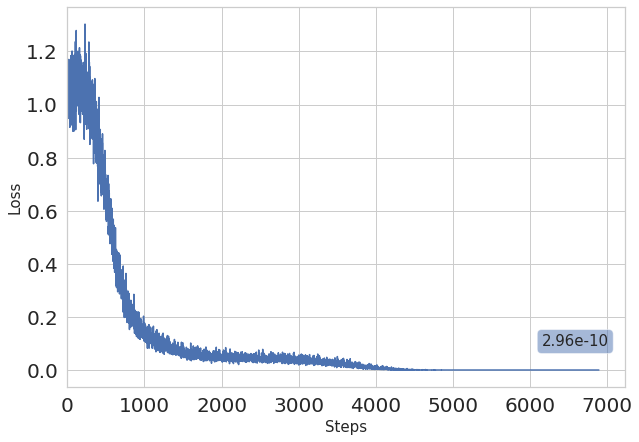
\includegraphics[height=5.9cm]{images/5j0n_perfect_angle_recovery.png}
        %\caption{Asymmetric protein (\texttt{5j0n}).}
    %\end{subfigure}
    %\hfill
    %\begin{subfigure}[b]{0.5\textwidth}
    %\centering
    %    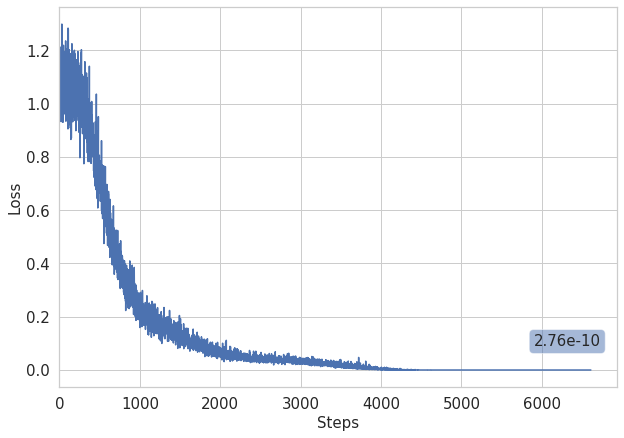
\includegraphics[height=5.5cm]{images/5a1a_perfect_angle_recovery.png}
    %    \caption{Symmetric protein (\texttt{5a1a}).}
    %\end{subfigure}
    \caption{Orientation recovery loss $d_p(\p_i, \p_j) = d_q(q_i, q_j)$ of the asymmetric protein (\texttt{5j0n}).} %\mdeff{Is it worth having the two here?}}
    \label{fig:5j0n-orientation-recovery-loss}
\end{figure}

Empirically we find that the mean orientation recovery error \eqnref{orientation-recovery-error} $E = 0$. The sphere coverage before and after the orientation alignment can be seen in the \figref{5j0n-aa-loss-perfect-distances}. We can see that the orientation alignment was performed successfully.
% \begin{figure}
%     \centering
%     \begin{subfigure}[b]{0.45\textwidth}
%         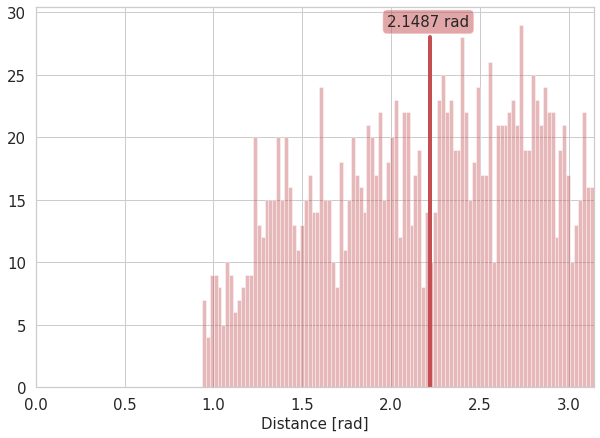
\includegraphics[height=5.7cm]{images/5j0n_perfect_angle_ralignment_before.png}
%         \caption{Before the alignment}
%     \end{subfigure}
%     \hfill
%     \begin{subfigure}[b]{0.5\textwidth}
%     \centering
%         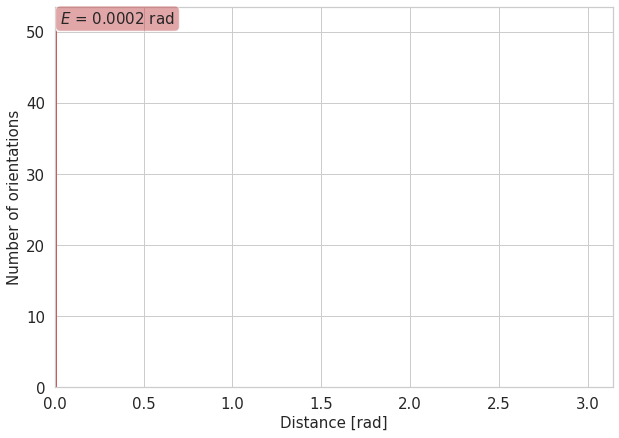
\includegraphics[height=5.7cm]{images/5j0n_perfect_angle_ralignment_after.png}
%         \caption{After the alignment}
%     \end{subfigure}
%     \caption{Example of perfect alignment: mean orientation error of true distances for asymmetric protein (\texttt{5j0n}) before and after the alignment.

%     }
%     \label{fig:angle-alignment-perfect}
% \end{figure}

\begin{figure}
    \centering
    \begin{subfigure}[b]{0.45\textwidth}
        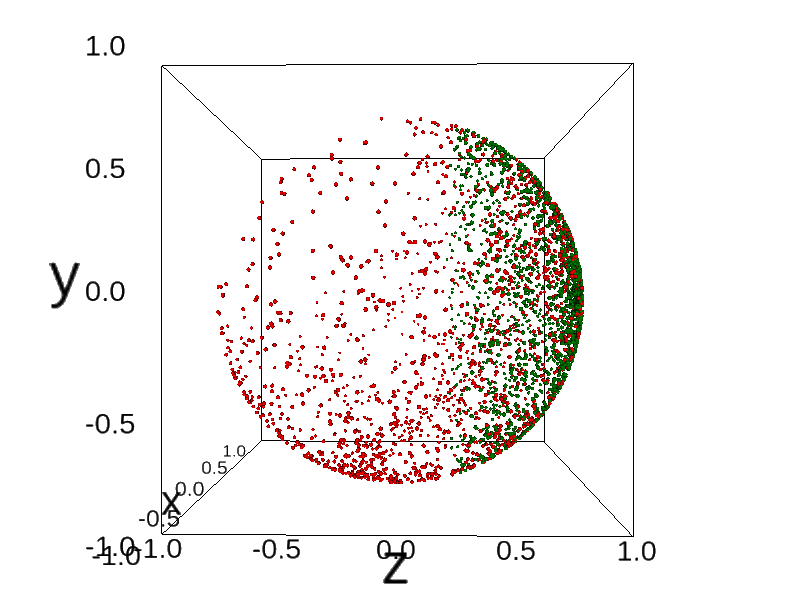
\includegraphics[height=6cm]{images/coverage_alignment_before.png}
        \caption{Before alignment \eqnref{orientation-recovery-error}.}
    \end{subfigure}
    \hfill
    \begin{subfigure}[b]{0.50\textwidth}
    \centering
        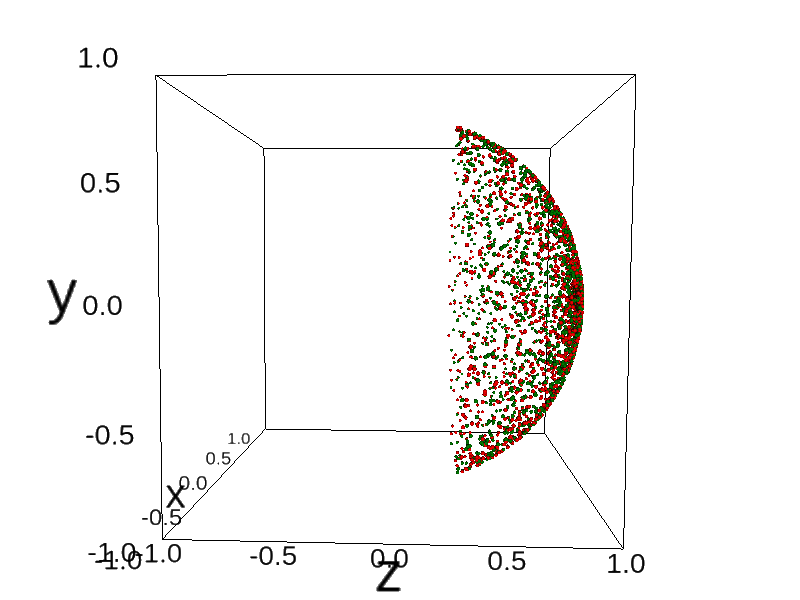
\includegraphics[height=6cm]{images/coverage_alignment_after.png}
        \caption{After alignment \eqnref{orientation-recovery-error}.}
    \end{subfigure}
    \caption{
        Orientation coverage of $\mathbb{S}^2 \subset \SO(3)$ after recovery.
        Green are ground truth orientations and red are estimated orientations.
        % orientations projected on S²
}
    \label{fig:5j0n-aa-loss-perfect-distances}
\end{figure}


%\subsubsection{Robustness of Recovery to Additive Errors on the Relative Distances}
\subsubsection{Sensitivity to distance estimation error}\label{sec:results:orientation-recovery:sensitivity}

%\mdeff{Story: (i) orientation recovery error is strongly linked to distance estimation error, (ii) recovery loss is a good proxy of mean recovery error.}

We now go one step further and evaluate the behaviour of~\eqnref{orientation-recovery} when the true relative distances are corrupted by additive Gaussian noise.

The experimental conditions are the same than in the previous section, except that we add an error with increasing variance on the relative distances prior to the minimization.
The results are presented in \figref{perfect-with-noise-ar-aa} (red curve).
For all variances, the mean orientation recovery error $E$ is reported in \figref{perfect-with-noise-ar-aa} (blue curve).


\begin{figure}[b]
    \centering
    \begin{subfigure}[b]{0.48\textwidth}
        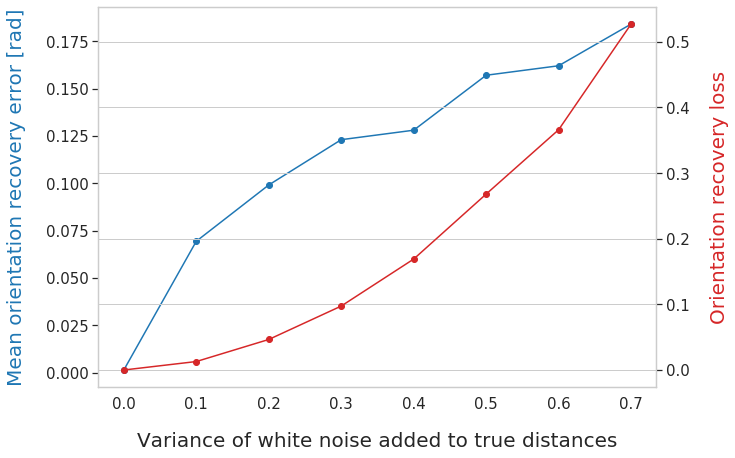
\includegraphics[height=5.15cm]{images/5j0n_perfect_noisy_ar_aa.png}
        \caption{Asymmetric protein (\texttt{5j0n}).}
    \end{subfigure}
    \hfill
    \begin{subfigure}[b]{0.50\textwidth}
    \centering
        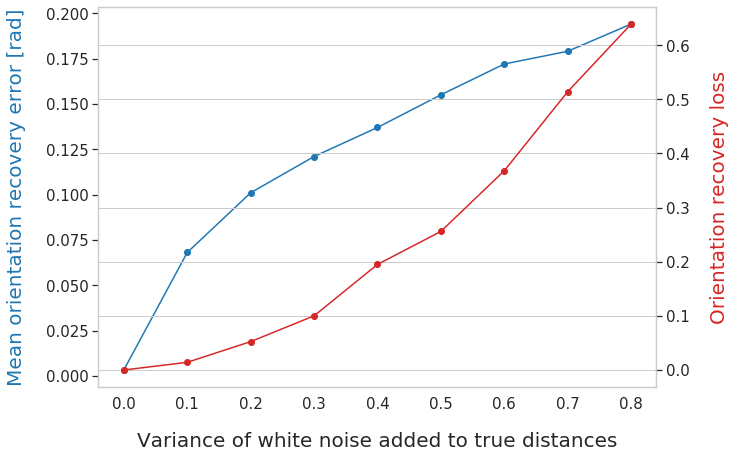
\includegraphics[height=5.15cm]{images/5a1a_perfect_noisy_ar_aa.png}
        \caption{Symmetric protein (\texttt{5a1a}).}
    \end{subfigure}
    \caption{
    The mean orientation recovery error \eqnref{orientation-recovery-error} is a monotonic function of the distance estimation error.
        Better distance estimation leads to better orientation recovery.
        Moreover, the recovery loss \eqnref{orientation-recovery} is a good proxy for the recovery error $E$, allowing us to assess recovery performance without ground-truth orientations.
}
    \label{fig:perfect-with-noise-ar-aa}
\end{figure}


These results demonstrate that the performance of the minimization scheme~\eqnref{orientation-recovery} linearly depends on the quality of the relative distances, which advocates for a proper and extensive training of the SiameseNN in the next stages of development.
Another interesting output of \figref{perfect-with-noise-ar-aa} is that it indicates that the error of the orientation recovery behaves as a monotonic function of its loss.
Hence, it suggests that the loss can be used as a good indicator of its performance, which has obvious practical implications for our future works on real data.


%%%%%%%%%%%%%%%%%%%%%%%%%%%%%%%%%%%%%%%%%%%%%%%%%%%%%%%%%%%%%%%%%%%%%%%%%%%%%%%%%%%%%%%
\subsection{Distance estimation}\label{sec:results:distance-estimation}
%\subsection{Estimating Relative Orientations from Projections}
%\subsection{Relative orientation estimation}

%\mdeff{Story: $d_p$ good estimator of $d_q$.
%SiameseNN better than l2, but still plateaus.
%Robust to projection noise.}

The challenge of distance estimation is to define the distance between two projections $d_p$ such that it is connected to the distance between two quaternions $d_q$. We start by using the Euclidean distance as the baseline. Then, we learn the distance metric using the SiameseNN architecture. With this network we aim to classify the new unseen pairs of projections without training the network again. Afterwards, we explore different network architectures as well as test the sensitivity of the network to perturbed projections.

%\mdeff{Could we quickly try translations? Should be no problem for Siamese.}


\subsubsection{Euclidean distance}\label{sec:results:distance-estimation:euclidean}

%\mdeff{Story: simplest baseline estimator, $d_{pe}$ somewhat estimates $d_q$, quickly plateaus (even in the simplest noiseless and centered case).
%Note the difference between symmetric and asymmetric proteins.}

As a baseline, we first evaluate the suitability of the Euclidean distance as a projection distance $d_p$ to predict $d_q$.
From $P = 5,000$ possible projection, we randomly select $5$ projections.
For each of these projections, we compute the Euclidean distance between aforementioned projection and all the others $d_p(\mathbf{p}_i,\mathbf{p}_j)=\lVert\mathbf{p}_i-\mathbf{p}_j\rVert_2$ and their corresponding orientation distance $d_q(q_i,q_j)$ through~\eqnref{distance:orientations}.
We then report the $(d_q,d_p)$ relationship for all pairs in \figref{euclidean-not-robust}, for both the asymmetric protein (left) and the symmetric one (right).

\begin{figure}[ht!]
    \centering
    \begin{subfigure}[t]{0.45\textwidth}
        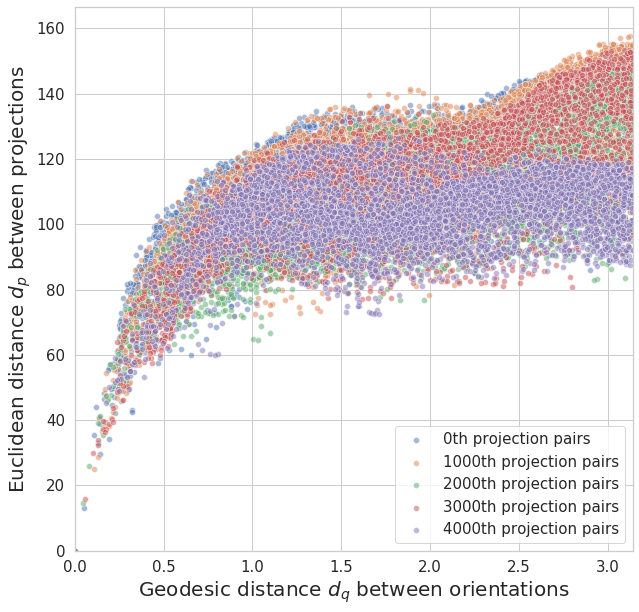
\includegraphics[height=7.5cm]{images/eucl_notrobust_5j0n.png}
        \caption{Asymmetric protein (\texttt{5j0n})}
    \end{subfigure} \quad \quad
    \begin{subfigure}[t]{0.5\textwidth}
        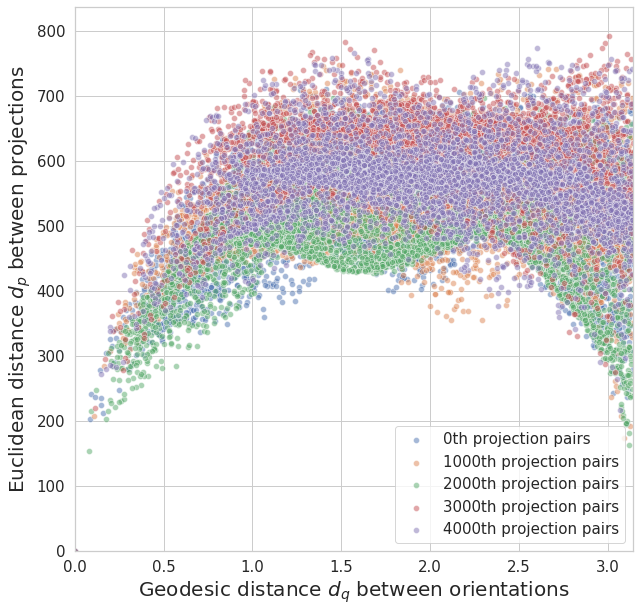
\includegraphics[height=7.5cm]{images/eucl_notrobust_5a1a.png}
        \caption{Symmetric protein (\texttt{5a1a})}
    \end{subfigure}
    \caption{Plotting the Euclidean distance between two projections versus their actual relative orientation (measured by the geodesic distance) for \textbf{(left)} the asymmetric protein (\texttt{5j0n}) dataset, and \textbf{(right)} the symmetric protein (\texttt{5a1a}) dataset. The color corresponds to projection pairs that share the first projection \textit{i.e.} distance between one projection with all other projections.}
    \label{fig:euclidean-not-robust}
\end{figure}


Two principal observations can be made from this experiment.
First, as suspected, the Euclidean distance between projections fails to be a consistent predictor of their relative orientation distance, even in the simple imaging conditions considered here (no noise and no effect of the PSF).
In particular, the larger the quaternion distance $d_q$, the poorer the predictive ability of the Euclidean distance as $d_p$.
The other interesting observation is that the intrinsic symmetry of the $\beta$-galactosidase protein (\texttt{5a1a}) appears in its $(d_q,d_p)$ plot.

\subsubsection{Learned distance}\label{sec:results:distance-estimation:learned}

%\mdeff{Story: learned distance $d_{ps}$ estimates $d_q$ with some variance but still underestimates larger distances.
%Again symmetric vs asymmetric.}


We present here a preliminary evaluation of the ability of SiameseNNs to learn a projection distance $\widehat{d}_p$ that correctly approximates the orientation distance $d_q$.

SiameseNNs come with a variety of more or less powerful architectures.
At the current stage of development, we work with a simple one.
Our SiameseNN is composed of two convolutional neural networks (CNNs) with shared weights.
Their output features vectors are compared through an Eulidean distance, \textit{i.e.}, $F(\mathbf{x},\mathbf{y})=\lVert \mathbf{x}-\mathbf{y}\rVert_2$ in \figref{schematic:distance-learning}.
Besides the Euclidean distance, this distance metric $F$ can be defined as geodesic distance, or it could be parametrized as MLP, used for a general function approximation, which we will explore in some of the following experiments.


\begin{figure}[ht!]
    \centering
    \begin{subfigure}[t]{0.45\textwidth}
        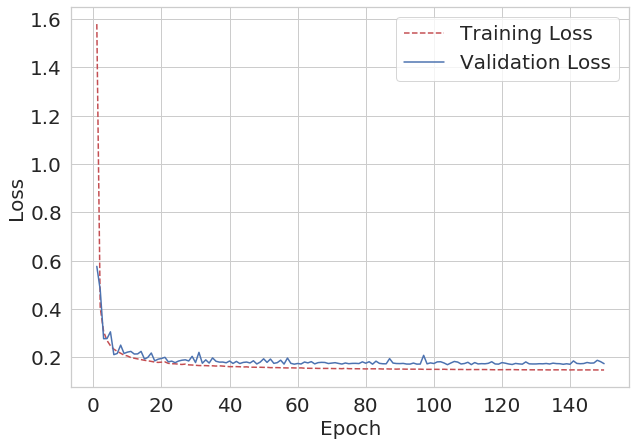
\includegraphics[height=5.5cm]{images/de_5j0n.png}
        \caption{Asymmetric protein (\texttt{5j0n})}
        \label{fig:losses-siamese-assym}
    \end{subfigure} \quad \quad
    \begin{subfigure}[t]{0.5\textwidth}
        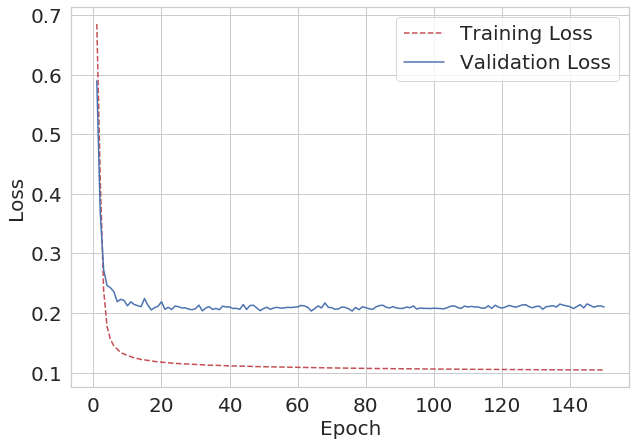
\includegraphics[height=5.5cm]{images/de_5a1a.png}
        \caption{Symmetric protein (\texttt{5a1a})}
        \label{fig:losses-siamese-sym}
    \end{subfigure}
    \caption{Distance estimation losses on the train and validation datasets.}
    \label{fig:losses-siamese}
\end{figure}

\begin{figure}
    \centering
    \begin{subfigure}[b]{0.45\textwidth}
        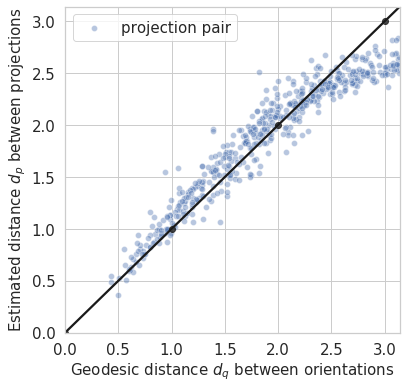
\includegraphics[height=6cm]{images/dPdQ_5j0n.png}
        \caption{Asymmetric protein (\texttt{5j0n}) on test dataset}
    \end{subfigure}
    \hfill
    \begin{subfigure}[b]{0.50\textwidth}
    \centering
        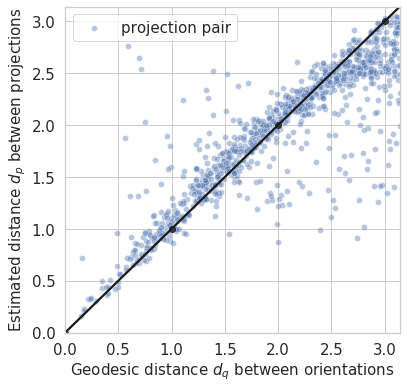
\includegraphics[height=6cm]{images/dPdQ_5a1a.png}
        \caption{Symmetric protein (\texttt{5a1a}) on test dataset}
    \end{subfigure}
    \caption{Relationship between orientations' distance $d_q$ and estimated distance $d_p$.}
    \label{fig:learned-distance-siamese}
\end{figure}


For each protein, we train the SiameseNN on its training dataset for 150 epochs ($\sim$2.6 hours) using an RMSProp optimizer~\cite{noauthor_tfkerasoptimizersrmsprop_nodate}, a learning rate of $10^{-3}$, and a batch size of 256 projections.
Depending on the available resources on the Google Colab, the training can last from 2.6 hours to 9.3 hours on one of its GPUs.
The evolution of the training and validation losses are presented in \figref{losses-siamese-assym} for the asymmetric protein (\texttt{5j0n}), and in \figref{losses-siamese-sym} for the symmetric one (\texttt{5a1a}).
The results demonstrate that the SiameseNN succeeds at learning a proxy distance for the asymmetric protein dataset, as convergence is reached in about 50 epochs ($\sim$ 50 minutes in the best resource availability setting).

However, the current SiameseNN architecture slightly overfits at learning the distance for the dataset \texttt{5a1a}, which is very likely due to the symmetry of the $\beta$-galactosidase protein, even thought the quarter-sphere coverage was used.
Indeed, its synthetic dataset may contain pairs of projections that share the same $d_p$, yet differ in their $d_q$.
This simply advocates for the restriction to non-overlapping areas on $\SO(3)$ when sampling the orientations used to generate the SiameseNN training dataset.
The latter would then only contain projection pairs with a linear $(d_q,d_p)$ relationship, which should ensure a successful training of the network.
For the rest of the experiments, we use the asymmetric protein (\texttt{5j0n}) dataset. Besides using the asymmetric protein, we will perform the full protein reconstruction pipeline on the symmetric protein (\texttt{5a1a}).

We then feed to the trained SiameseNN $1,000$ pairs of projections randomly selected from the \texttt{5j0n} testing dataset, and report the $(d_q,\widehat{d}_p)$ relationship of each pair in \figref{learned-distance-siamese}.
These results confirm that, the SiameseNN is able to predict the orientation distance $d_q$ using only the projections as inputs. The prediction performance is slightly better for the asymmetric protein compared to symmetric protein.
Moreover, it clearly outperforms the Euclidean distance at doing so.
These preliminary results are encouraging, as much has yet to be gained from improving upon the rather primitive SiameseNN architecture we currently use. The architecture of implemented SiameseNN can be seen in Appendix~\ref{sec:siamese-architecture}.

\subsubsection{Influence of network architecture and feature distance}

%\mdeff{Story: $d_f = d_q$ better than Euclidean and MLP $d_f$. Architecture of $G_w$ doesn't seem to matter much. Surprising, because we don't overfit $\rightarrow$ future research needed.}

To further improve our network, we experiment with different feature distance metrics $F(\mathbf{x},\mathbf{y})$.
In the previous experiments we used the Euclidean distance as a features distance metric, \textit{i.e.} $F(\mathbf{x},\mathbf{y})=\lVert \mathbf{x}-\mathbf{y}\rVert_2$.

In this experiment, we test the performance with a geodesic distance, \textit{i.e.}
\begin{equation}
    F(\mathbf{x},\mathbf{y})=2 \arccos(\frac{\mathbf{x} \cdot \mathbf{y}}{\lVert \mathbf{x} \rVert \lVert \mathbf{y} \rVert}) = 2 \arccos(\frac{\sum_{i=1}^n x_i y_i}{\sqrt{\sum_{i=1}^n x_i^2}\sqrt{\sum_{i=1}^n y_i^2 }}).
    \label{eqn:geodesic-distance}
\end{equation}

Additionally, we parametrize $F(\mathbf{x},\mathbf{y})$ as MLP. It consists of six hidden linear layers with \texttt{1024}, \texttt{512}, \texttt{512}, \texttt{256}, \texttt{256}, and \texttt{1} unit respectively. All of them use SeLU as an activation function.

The experimental conditions are the same as in the previous section with the Euclidean distance metric as feature distance metric.
\figref{geo-eucl-mlp} shows the training and validation losses of the geodesic distance are better than Euclidean and MLP feature distance metric. We can also observe the performance on the $(d_q, d_p)$ plots and notice that the projection pairs deviate the least using the geodesic distance.

\begin{figure}
    \centering
    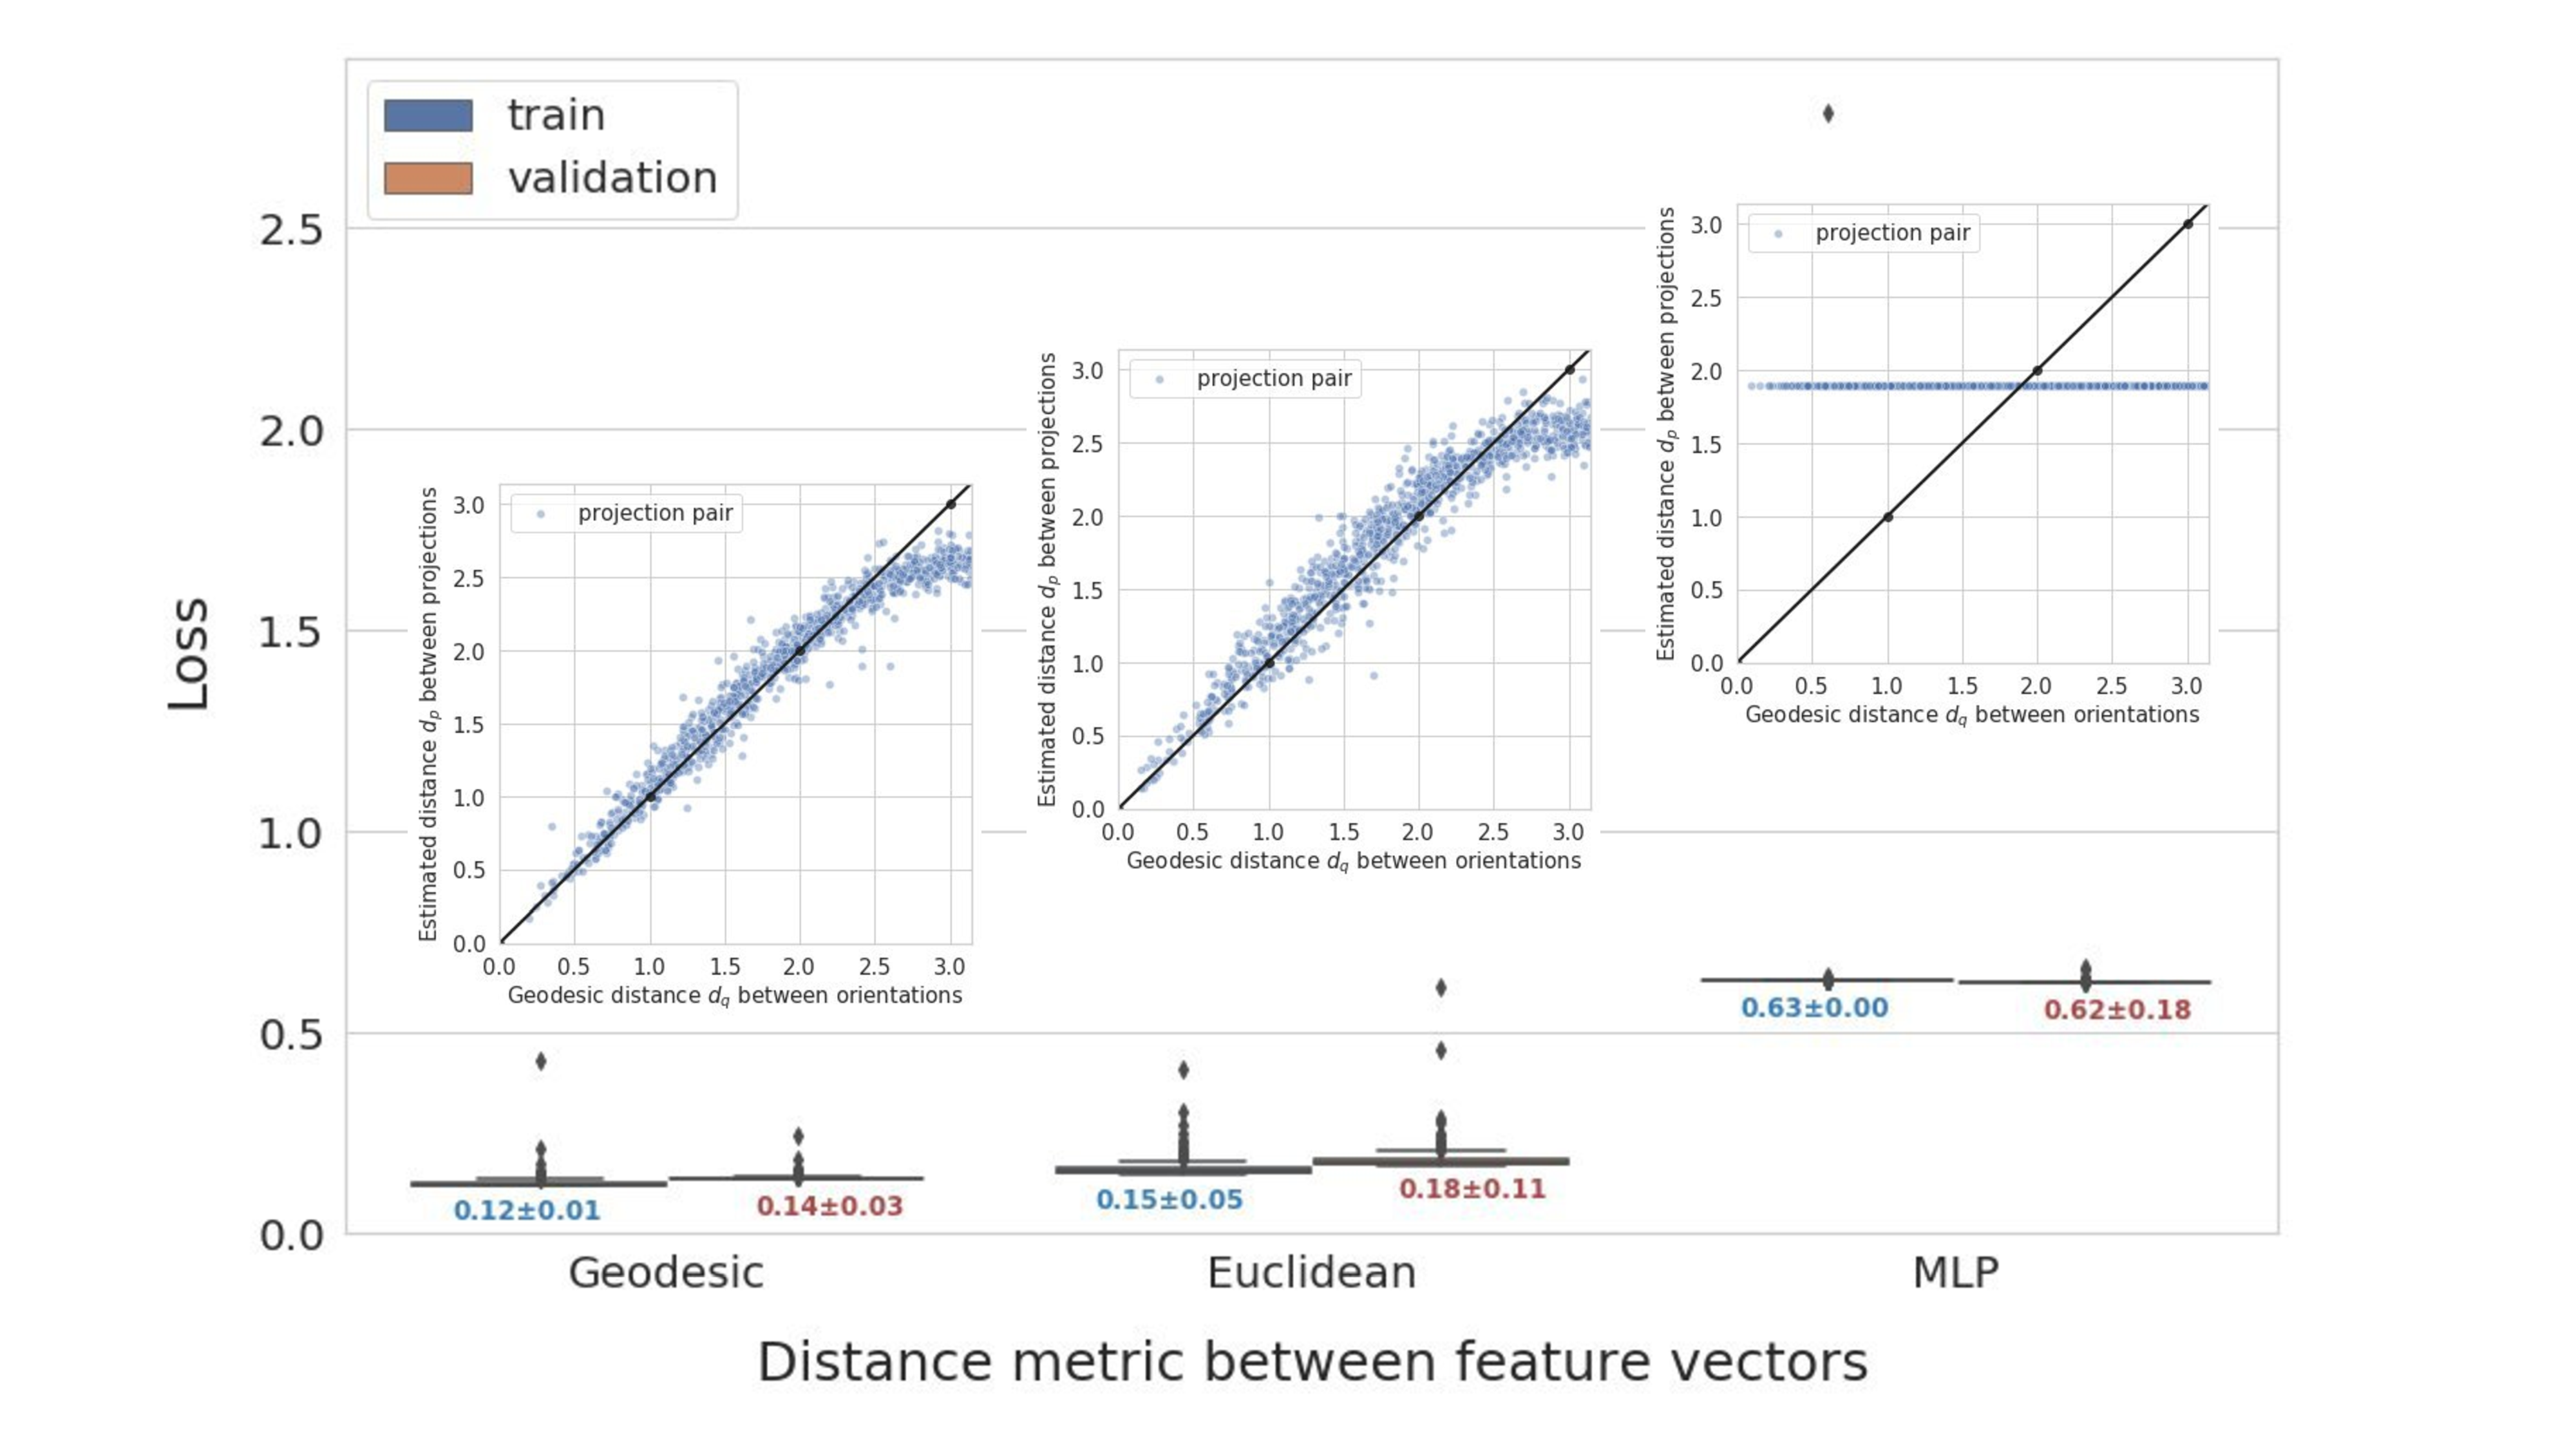
\includegraphics[height=8.5cm]{images/geo_eucl_mlp_distance_metric.pdf}
    \caption{Training and validation losses w.r.t. feature vectors' distance metric and their corresponding distance ratio $(d_q, d_p)$ plots.}
    \label{fig:geo-eucl-mlp}
\end{figure}


\subsubsection{Sensitivity to perturbed projections}\label{sec:results:distance-estimation:sensitivity}

%\mdeff{Story: learned distance is minimally sensible to perturbations (additive noise, translation, PSF) because we can train it to ignore irrelevant information.
%Thanks again to good model of cryo-EM imaging.}
%\mdeff{Better word? (perturbations, quality, non-ideal)}

In this experiment we want to explore how does the perturbation of the projections affect the distance estimation (additive noise, translation, PSF).

The experimental conditions for the experiment are the same as before, except that we add noise with increasing variance on the projection prior to training.
The results are presented in \figref{distance-estimation-vary-projection-noise}.

We observe that the training and validation losses are increasing and network starts to overfit w.r.t. amount of noise in the projections.
With the noiseless projections (projection noise variance 0), the mean orientation recovery error $E = 0.1594$ rad.
Whereas, the noisy projections with noise levels 15 are the closest to the realistic protein projections and the error $E=4189$ rad.

Besides testing the performance of the pipeline with the noisy projections, we explore the performance with different projection translation levels.
To translate the projection, we use a triangular distribution from $-t$ to $t$ px translation with the peak in the center of the projection.
The performance of different translation magnitudes can be seen in \figref{distance-estimation-vary-projection-translation}.
We observe that the training of the network is invariant to translations in the projections, which was expected.

We can see that the learned distance is minimally sensible to perturbations because we can train the network to ignore irrelevant information.

\begin{figure}[ht!]
    \centering
        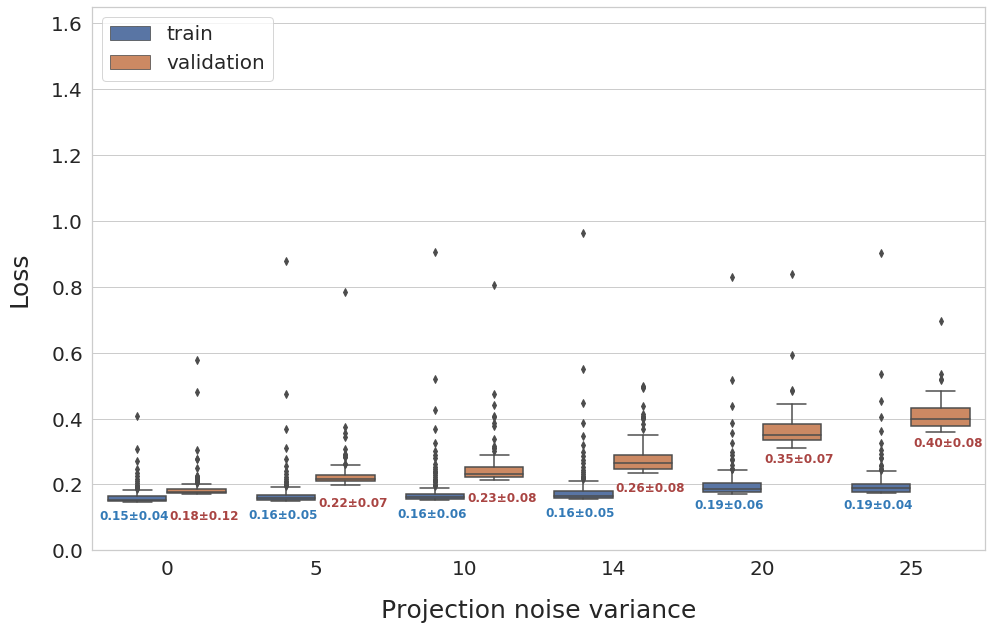
\includegraphics[height=8cm]{images/de_noises_nums.png}
        \caption{%
            Variation of train and validation epoch losses w.r.t. noise levels in the projections of the asymmetric protein (\texttt{5j0n}). The mean orientation recovery error $E$ is in the red box, and the orientation recovery loss $OR$ is in the blue box.
        }\label{fig:distance-estimation-vary-projection-noise}
\end{figure}

\begin{figure}
    \centering
        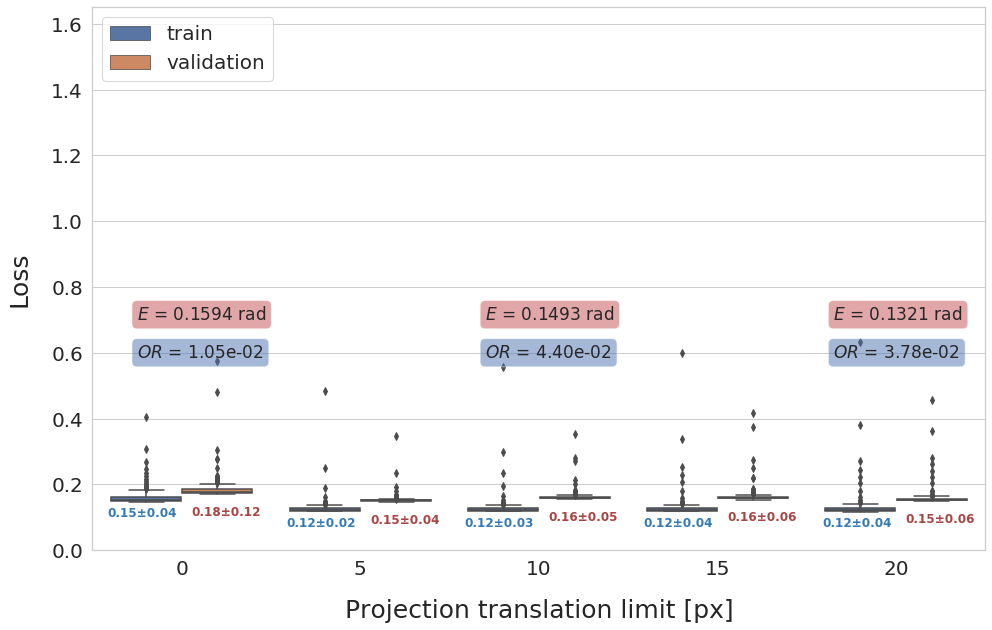
\includegraphics[height=8cm]{images/de_translation_nums.png}
        \caption{
        Variation of train and validation epoch losses w.r.t.\ projection translation of the asymmetric protein (\texttt{5j0n}). The mean orientation recovery error $E$ is in the red box, and the orientation recovery loss $OR$ is in the blue box.
    }\label{fig:distance-estimation-vary-projection-translation}
\end{figure}


\subsection{Orientation recovery from estimated distances}

%\mdeff{Story: pipeline works but better distance estimation is needed for SOTA reconstruction.
%Method is however promising because learned distance is robust to perturbations and recovery works if distance works.}
%\todo{Justify threshold because of plateau (figref).
%Show recovered orientations w.r.t.\ ground truth after alignment.}
%\todo{Reconstruct the protein to show the full pipeline: from a set of projections to a reconstructed protein.
%Emphasize that it's a naive reconstruction algorithm.}

The orientation recovery from estimated distances represents a full pipeline needed to reconstruct the protein from a given set of projections.
We run the pipeline for both, asymmetric (\texttt{5j0n}) and symmetric (\texttt{5a1a}) protein.
In addition, we run the pipeline for the simulated realistic noise in the asymmetric protein.
The experimental setting for distance estimation is the similar to the one used to generate the \figref{learned-distance-siamese}: 150 epochs, 1e-3 learning rate, batch size 256 with random sampling of the projections, but for feature distance metric we use the geodesic distance since it showed the best performance in \figref{geo-eucl-mlp}.

Then, we run the orientation recovery on the estimated distances of the asymmetric protein and the performance results can be observed in \figref{5j0n-orientation-recovery-loss-est} with the same experimental setting as in \figref{5j0n-orientation-recovery-loss}.
With the noiseless projections, the objective function successfully converges to the $0.0510$ and with the noisy projections, the objective function converges to the $0.0683$.


\begin{figure}[ht!]
    \centering
    \begin{subfigure}[b]{0.45\textwidth}
        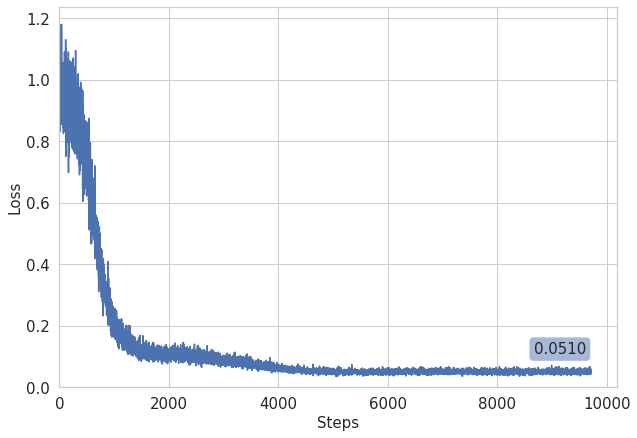
\includegraphics[height=5.5cm]{images/5j0n_noise0_angle_recovery.png}
        \caption{Noiseless projections}
    \end{subfigure}
    \hfill
    \begin{subfigure}[b]{0.5\textwidth}
    \centering
        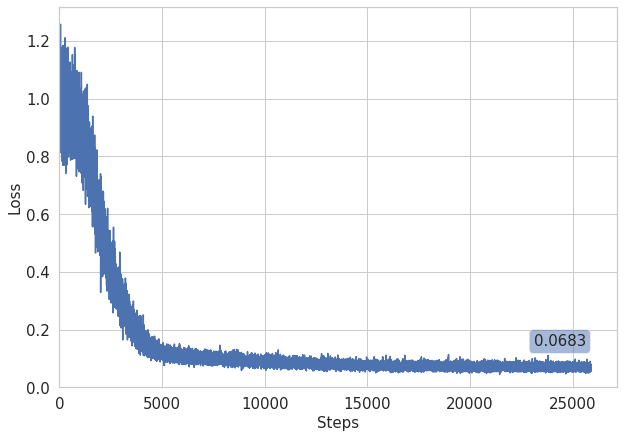
\includegraphics[height=5.5cm]{images/5j0n_noise16_angle_recovery.png}
        \caption{Noisy projections (variance 16)}
    \end{subfigure}
    \caption{ Orientation recovery loss of the asymmetric protein (\texttt{5j0n}).}
    \label{fig:5j0n-orientation-recovery-loss-est}
\end{figure}

The mean orientation recovery error for asymmetric protein \texttt{5j0n} without noise in the projection can be seen in \figref{angle-alignment-5j0n-noise0}.
Experimental setting parameters are: 3 runs per reflection/mirror (this is the $m=\det(\T)=1$ and $m=\det(\T)=-1$, therefore, total number of runs is 6), 300 steps, batch size 256, FTRL optimizer with learning rate 2.0 and learning rate power -2.0.
The smallest error achieved is $0.1594$ rad.

The mean orientation recovery error for asymmetric protein \texttt{5j0n} with noisy projections (white noise with variance 16) can be seen in \figref{angle-alignment-5j0n-noise16}. Experimental setting parameters are: 3 runs per reflection (total number of runs is 6), 300 steps, batch size 256, FTRL optimizer with learning rate 2.0 and learning rate power -2.0. The smallest error achieved is $0.4184$ rad.

\begin{figure}
    \centering
    \begin{subfigure}[b]{0.45\textwidth}
        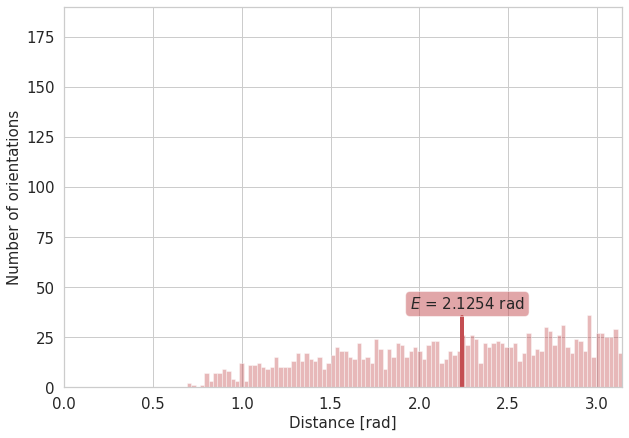
\includegraphics[height=5.7cm]{images/5j0n_noise0_angle_alignment_before.png}
        \caption{Arbitrary orientation error before the alignment.}
    \end{subfigure}
    \hfill
    \begin{subfigure}[b]{0.5\textwidth}
    \centering
        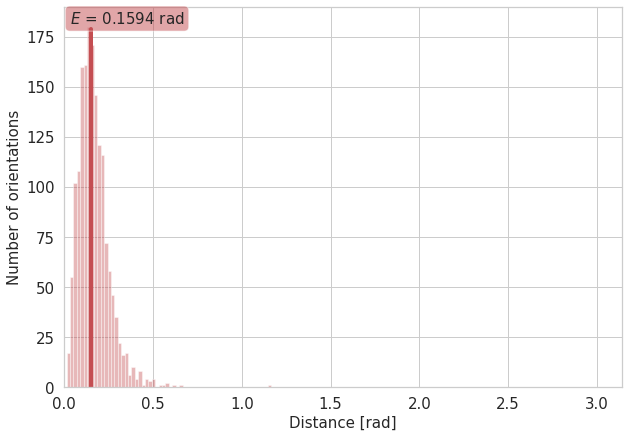
\includegraphics[height=5.7cm]{images/5j0n_noise0_angle_alignment_after.png}
        \caption{Minimal orientation error after the best alignment.}
    \end{subfigure}
    \caption{
        Mean orientation recovery error $E$ from equation \eqnref{orientation-recovery-error} for the asymmetric protein (\texttt{5j0n}).
    }
    \label{fig:angle-alignment-5j0n-noise0}
\end{figure}


\begin{figure}[ht!]
    \centering
    \begin{subfigure}[b]{0.45\textwidth}
        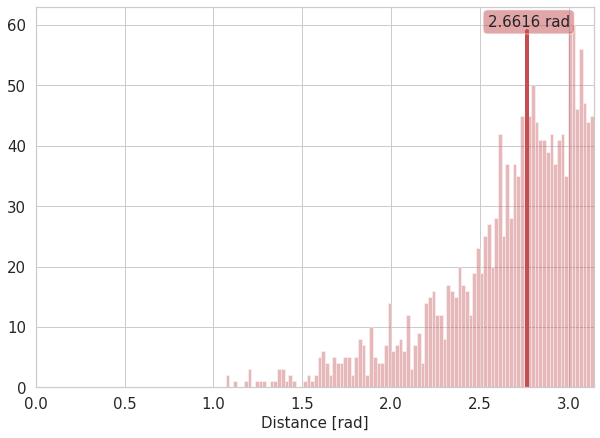
\includegraphics[height=5.7cm]{images/5j0n_noise16_angle_alignment_before.png}
        \caption{Arbitrary orientation error before the alignment.}
    \end{subfigure}
    \hfill
    \begin{subfigure}[b]{0.5\textwidth}
    \centering
        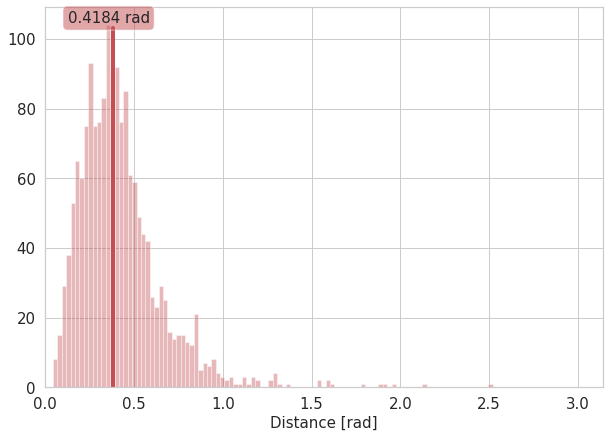
\includegraphics[height=5.7cm]{images/5j0n_noise16_angle_alignment_after.png}
        \caption{Minimal orientation error after the best alignment.}
    \end{subfigure}
    \caption{
        Mean orientation recovery error $E$ from equation \eqnref{orientation-recovery-error} of the asymmetric protein (\texttt{5j0n}) with white noise (variance 16).
}
    \label{fig:angle-alignment-5j0n-noise16}
\end{figure}

As a last step of the pipeline, we perform protein reconstruction using the projections and their corresponding estimated orientations.
For that, we again use the ASTRA toolbox.
Using this toolbox, we generate orientation vectors based on angles which we later feed into projection 3D geometry in ASTRA.
Due to GPU memory limit, we are able to reconstruct the protein using maximum of $3,000$ projections.
It holds for our case, since we perform orientation recovery on the test set which has in total $1,650$ projections (less than the limit of $3,000$).

The reconstruction results for the asymmetric protein (\texttt{5j0n}) with noiseless projections can be seen in \figref{5j0n-reconstruction-noise0}. On the left side we have a reconstruction using the ground-truth orientations, and on the right side we have the reconstruction result using the estimated aligned orientations.

\begin{figure}[ht!]
    \centering
    \begin{subfigure}[b]{0.45\textwidth}
        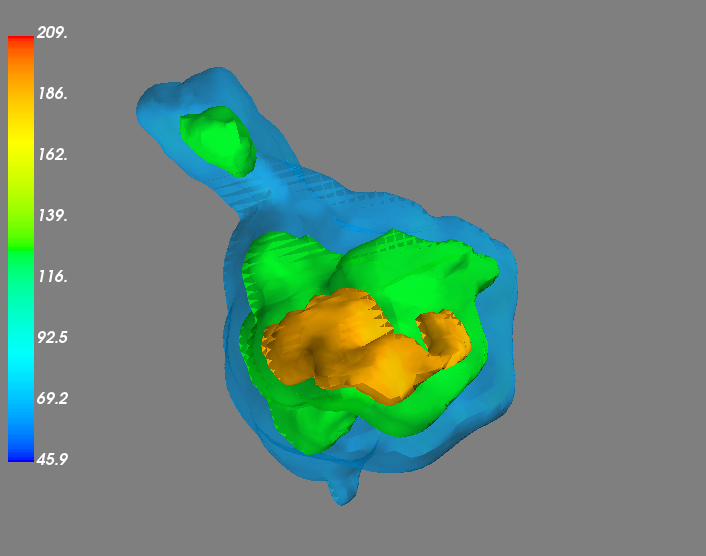
\includegraphics[height=5.5cm]{images/5j0n_reconstruction_GT.png}
        \caption{Ground truth.}
    \end{subfigure}
    \hfill
    \begin{subfigure}[b]{0.5\textwidth}
    \centering
        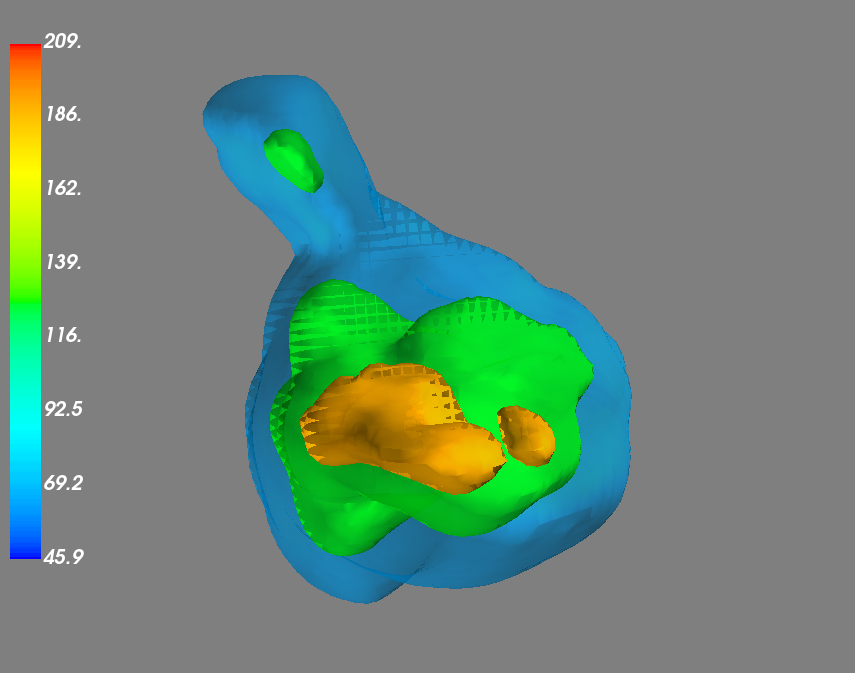
\includegraphics[height=5.5cm]{images/5j0n_reconstruction_noise0.png}
        \caption{Estimated.}
    \end{subfigure}
    \caption{
        Reconstruction of the asymmetric protein (\texttt{5j0n}).
    }\label{fig:5j0n-reconstruction-noise0}
\end{figure}

The reconstruction results for the asymmetric protein (\texttt{5j0n}) with noisy projections (with noise variance 16) can be seen in \figref{5j0n-reconstruction-noise16}.
Similarly, on the left side we have a reconstruction using the ground-truth orientations, and on the right side we have the reconstruction result using the estimated aligned orientations.

\begin{figure}[ht!]
    \centering
    \begin{subfigure}[b]{0.45\textwidth}
        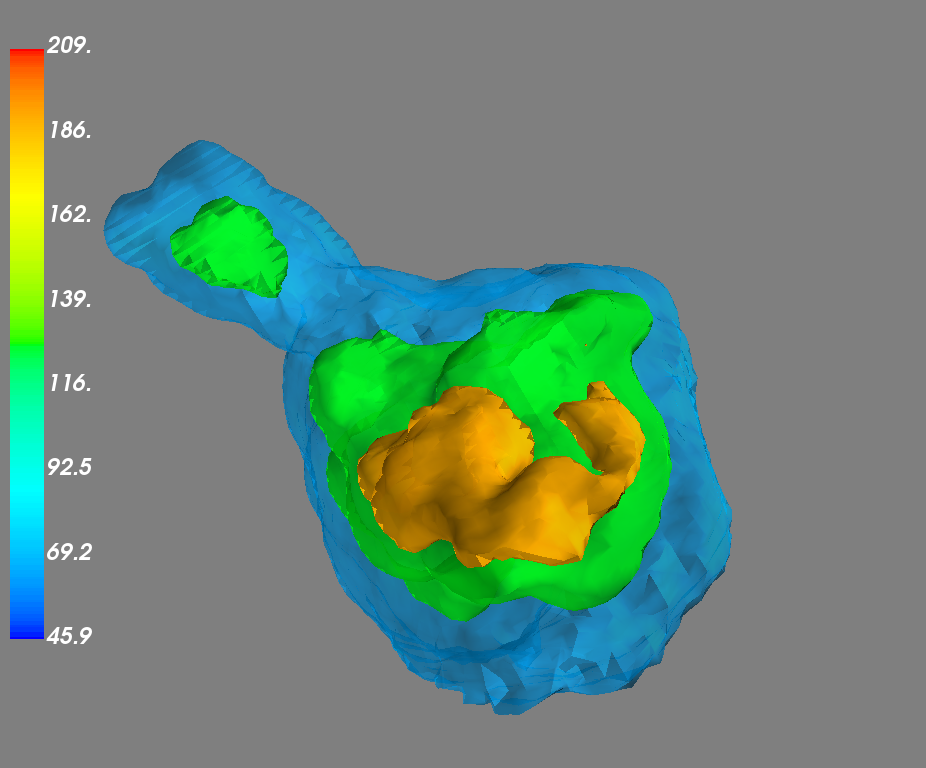
\includegraphics[height=5.5cm]{images/5j0n_reconstruction_GT_noise16.png}
        \caption{Ground truth.}
    \end{subfigure}
    \hfill
    \begin{subfigure}[b]{0.5\textwidth}
    \centering
        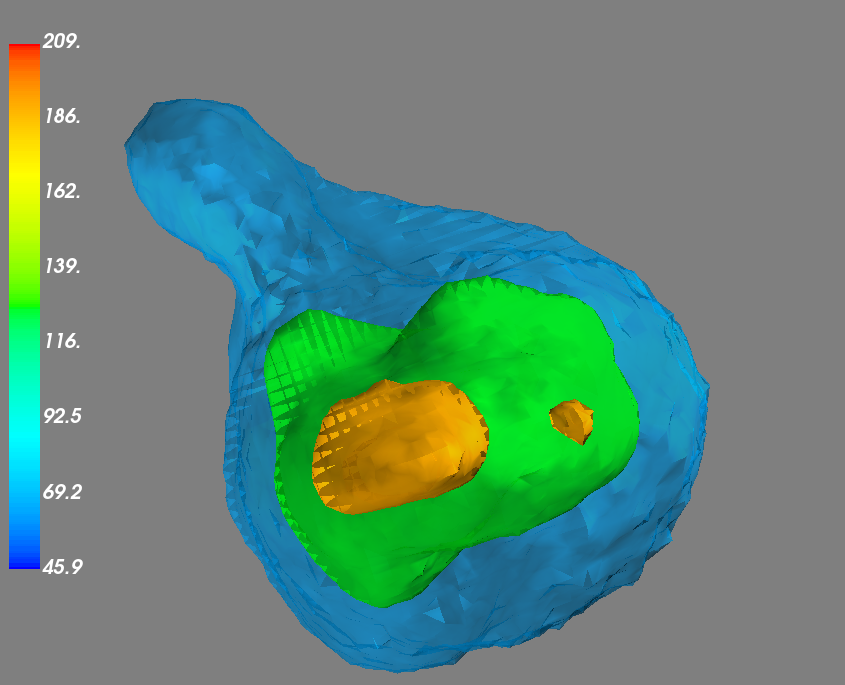
\includegraphics[height=5.5cm]{images/5j0n_reconstruction_noise16.png}
        \caption{Estimated.}
    \end{subfigure}
    \caption{
        Reconstruction of the asymmetric protein (\texttt{5j0n}) with noisy projections.
    }\label{fig:5j0n-reconstruction-noise16}
\end{figure}



%%%%%%%%%%% 5a1a

Similarly, we run the whole reconstruction pipeline on the symmetric protein (\texttt{5a1a}).
The experimental conditions for the distance estimation are the same as for the asymmetric protein, except that we use the quarter-sphere projections coverage (whereas, in the asymmetric protein we use half-sphere coverage).
The orientation recovery loss can be seen in \figref{5a1a-orientation-recovery-loss}. It successfully converges to $0.0381$.

\begin{figure}[ht!]
    \centering
    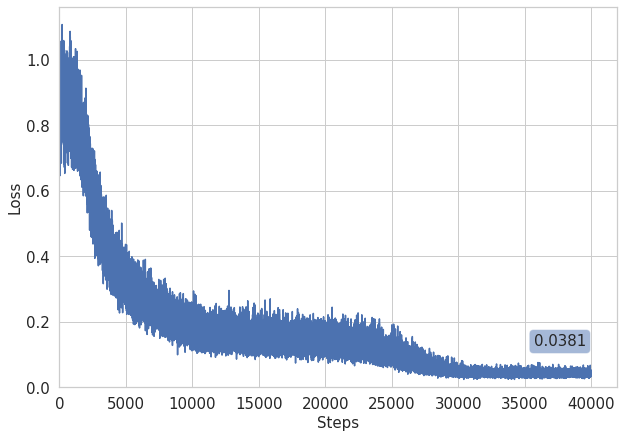
\includegraphics[height=5.5cm]{images/5a1a_noise0_angle_recovery.png}
    \caption{ Orientation recovery loss of the symmetric protein (\texttt{5a1a}).}
    \label{fig:5a1a-orientation-recovery-loss}
\end{figure}

The mean orientation recovery error for symmetric protein \texttt{5a1a} can be seen in \figref{angle-alignment-5a1a-noise0}. Experimental setting parameters are: 3 runs per reflection (total number of runs is 6), 300 steps, batch size 256, FTRL optimizer with learning rate 2.0 and learning rate power -2.0. The smallest error achieved is $0.1871$ rad.

\begin{figure}[ht!]
    \centering
    \begin{subfigure}[b]{0.45\textwidth}
        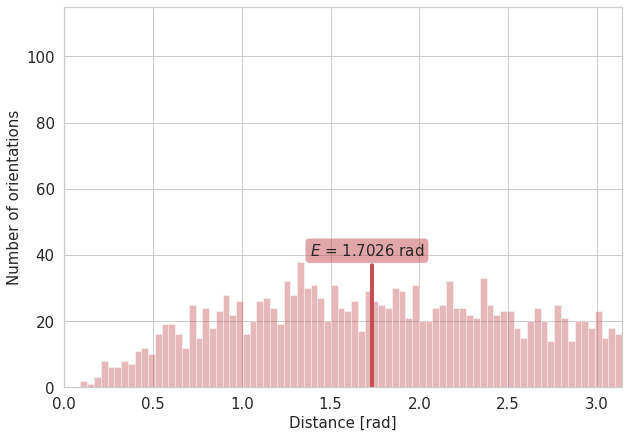
\includegraphics[height=5.7cm]{images/5a1a_noise0_angle_alignment_before.png}
        \caption{Arbitrary orientation error before the alignment.}
    \end{subfigure}
    \hfill
    \begin{subfigure}[b]{0.5\textwidth}
    \centering
        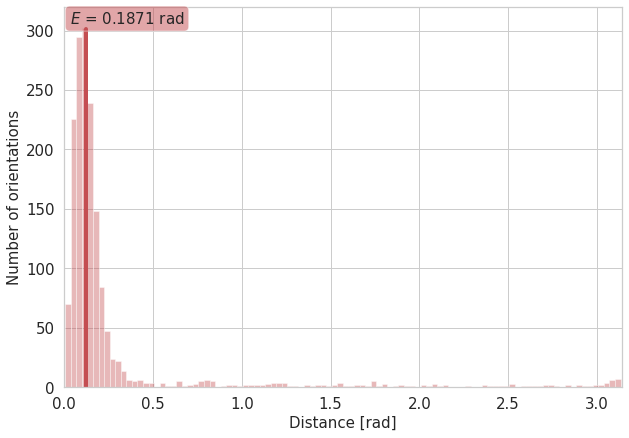
\includegraphics[height=5.7cm]{images/5a1a_noise0_angle_alignment_after.png}
        \caption{Minimal orientation error after the best alignment.}
    \end{subfigure}
    \caption{
        Mean orientation recovery error $E$ from equation \eqnref{orientation-recovery-error} for the symmetric protein (\texttt{5a1a}).
    }
    \label{fig:angle-alignment-5a1a-noise0}
\end{figure}

Lastly, we perform the protein reconstruction with the same ASTRA toolbox setting as for the asymmetric protein. The results of the reconstruction can be observed in the \figref{5a1a-reconstruction-noise0}.

\begin{figure}[ht!]
    \centering
    \begin{subfigure}[b]{0.45\textwidth}
        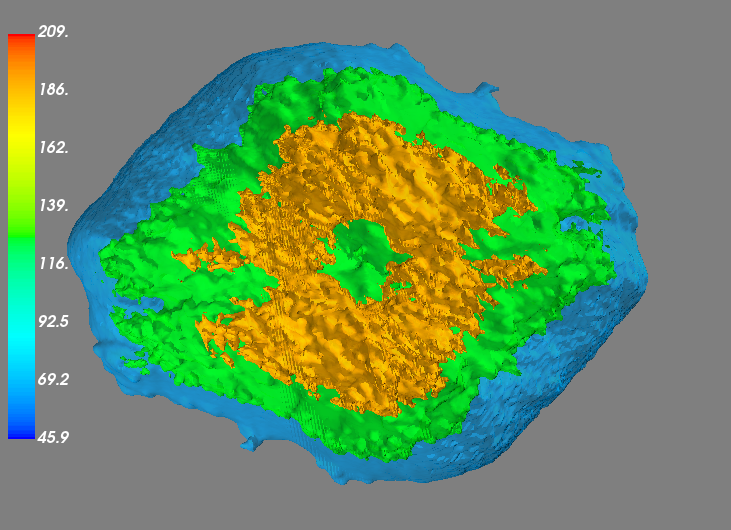
\includegraphics[height=5.5cm]{images/5a1a_ground_truth.png}
        \caption{Ground truth.}
    \end{subfigure}
    \hfill
    \begin{subfigure}[b]{0.5\textwidth}
    \centering
        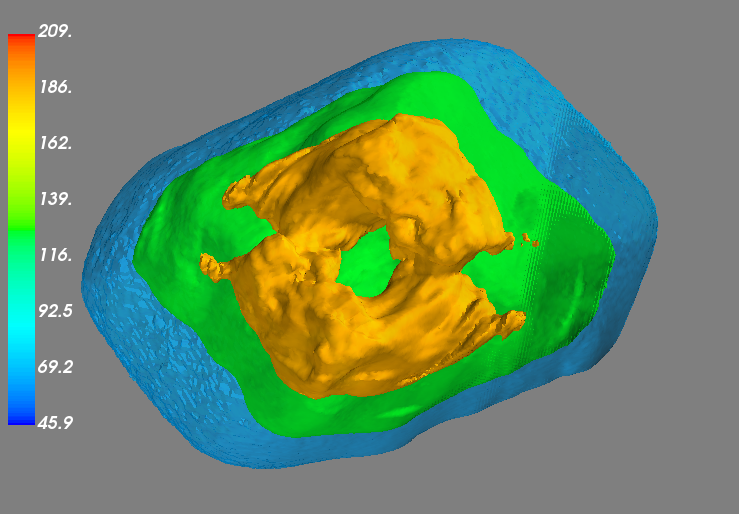
\includegraphics[height=5.5cm]{images/5a1a_aligned.png}
        \caption{Estimated.}
    \end{subfigure}
    \caption{
        Reconstruction of the symmetric protein (\texttt{5a1a}) with noisy projections.
    }\label{fig:5a1a-reconstruction-noise0}
\end{figure}

We were able to successfully reconstruct the symmetric protein even though the distance estimation was noisier than the one performed on the asymmetric protein.

We observe that the pipeline works, but for the state-of-the-art reconstruction we need a better distance estimation.
However, the method developed is promising since the learned distance is robust to perturbations.
We observe that the orientation recovery and distance estimation are interconnected, \textit{i.e.} if one works the other one will work.

